\newpage
\section{Punto 2}

\textit{Para buscar, mediante el algoritmo de Horspool, un patrón de longitud m en un texto de longitud n, con $n \leq m$, dar un ejemplo para: 
\begin{itemize}
  \item Mejor caso.
  \item Peor caso.
\end{itemize}
}

El algoritmo de Horspool es una version simplificada del algoritmo Boyer-Moore utilizando una única tabla. Este pre-procesa el patron que se desea encontrar generando una tabla de desplazamiento que determina cuanto desplazar el patron cuando ocurre un fallo \ref{fig:horspool tabla}.

\begin{figure}
  \centering
  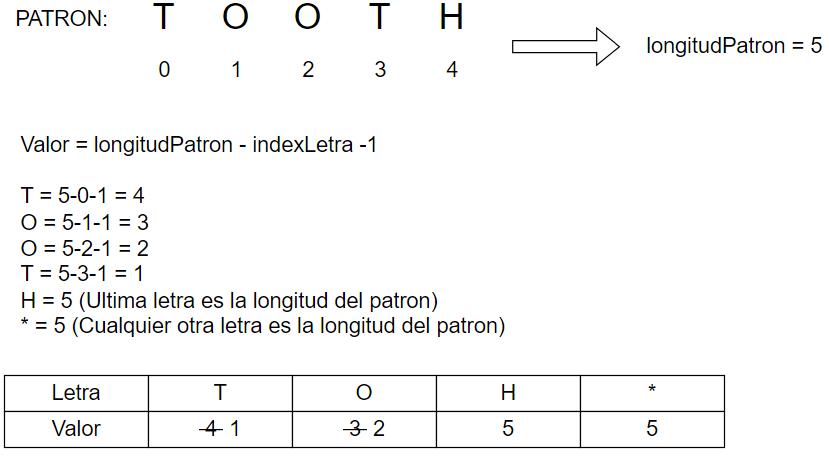
\includegraphics[width=\textwidth, scale=1]{Images/Punto2/Horspool Tabla.png}
  \caption{Ejemplo de creación de tabla de errores}
  \label{fig:horspool tabla}
\end{figure}

Siempre realizaran los desplazamientos basados en el carácter del texto c alineado con el ultimo carácter comparado (fallo) en el patron de acuerdo a la entrada a la tabla de desplazamiento para c \ref{fig:horspool traza}.\\

\begin{figure}[!htb]
  \centering
  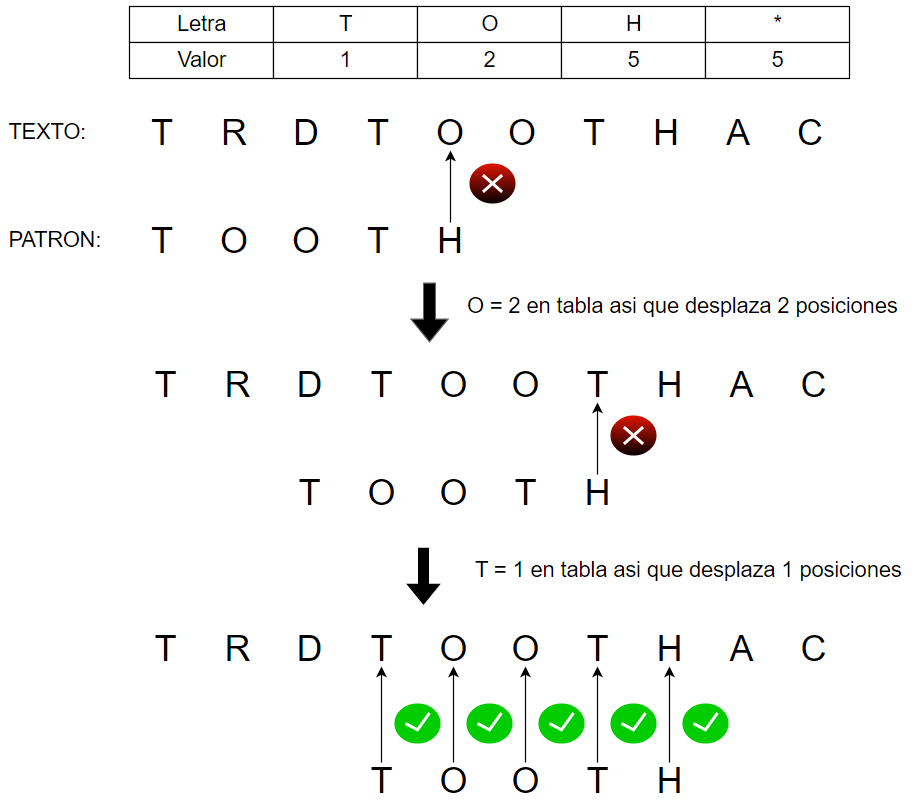
\includegraphics[width=\textwidth, scale=1]{Images/Punto2/Horspool traza.png}
  \caption{Traza de búsqueda de patron con algoritmo de Horspool}
  \label{fig:horspool traza}
\end{figure}


\textbf{Análisis de eficiencia:}
\begin{itemize}
  \item El peor caso sera un patron en el cual coinciden todos los caracteres excepto el primero por ejemplo:
  \begin{itemize}
    \item $1^n$ texto de entrada (longitud n)
    \item $0111\ldots 1$ patron (longitud m)
  \end{itemize}
  En este caso se chequearan constantemente los $m$ caracteres del patron por lo que se tendrá en el peor caso, es decir cuando se hagan desplazamientos de a una posición al encontrar el fallo, un tiempo de ejecución $O(nm)$.

  \item El mejor caso sera cuando el texto de entrada no contenga caracteres del patron por ejemplo:
  \begin{itemize}
    \item $1^n$ texto de entrada (longitud n)
    \item $0^m$ patron (longitud m)
  \end{itemize}
  esto hará que se produzcan saltos del tamaño del patron, es decir de tamaño $m$, produciendo un tiempo de ejecución $O(m/n)$.
\end{itemize}